
\chapter{Arquitetura de Software}
\label{sec-arquitetura}

A arquitetura de software do sistema~\imprimirtitulo\ segue a arquitetura padrão sugerida pelo FrameWeb~\cite{souza:masterthesis07,souza-et-al:iism09} baseada no padrão Camada de Serviço~\cite{fowler:book02}. A Figura~\ref{figura-arquitetura-padrao} ilustra a arquitetura estabelecida pelo método FrameWeb.

\begin{figure}[h]
	\centering
	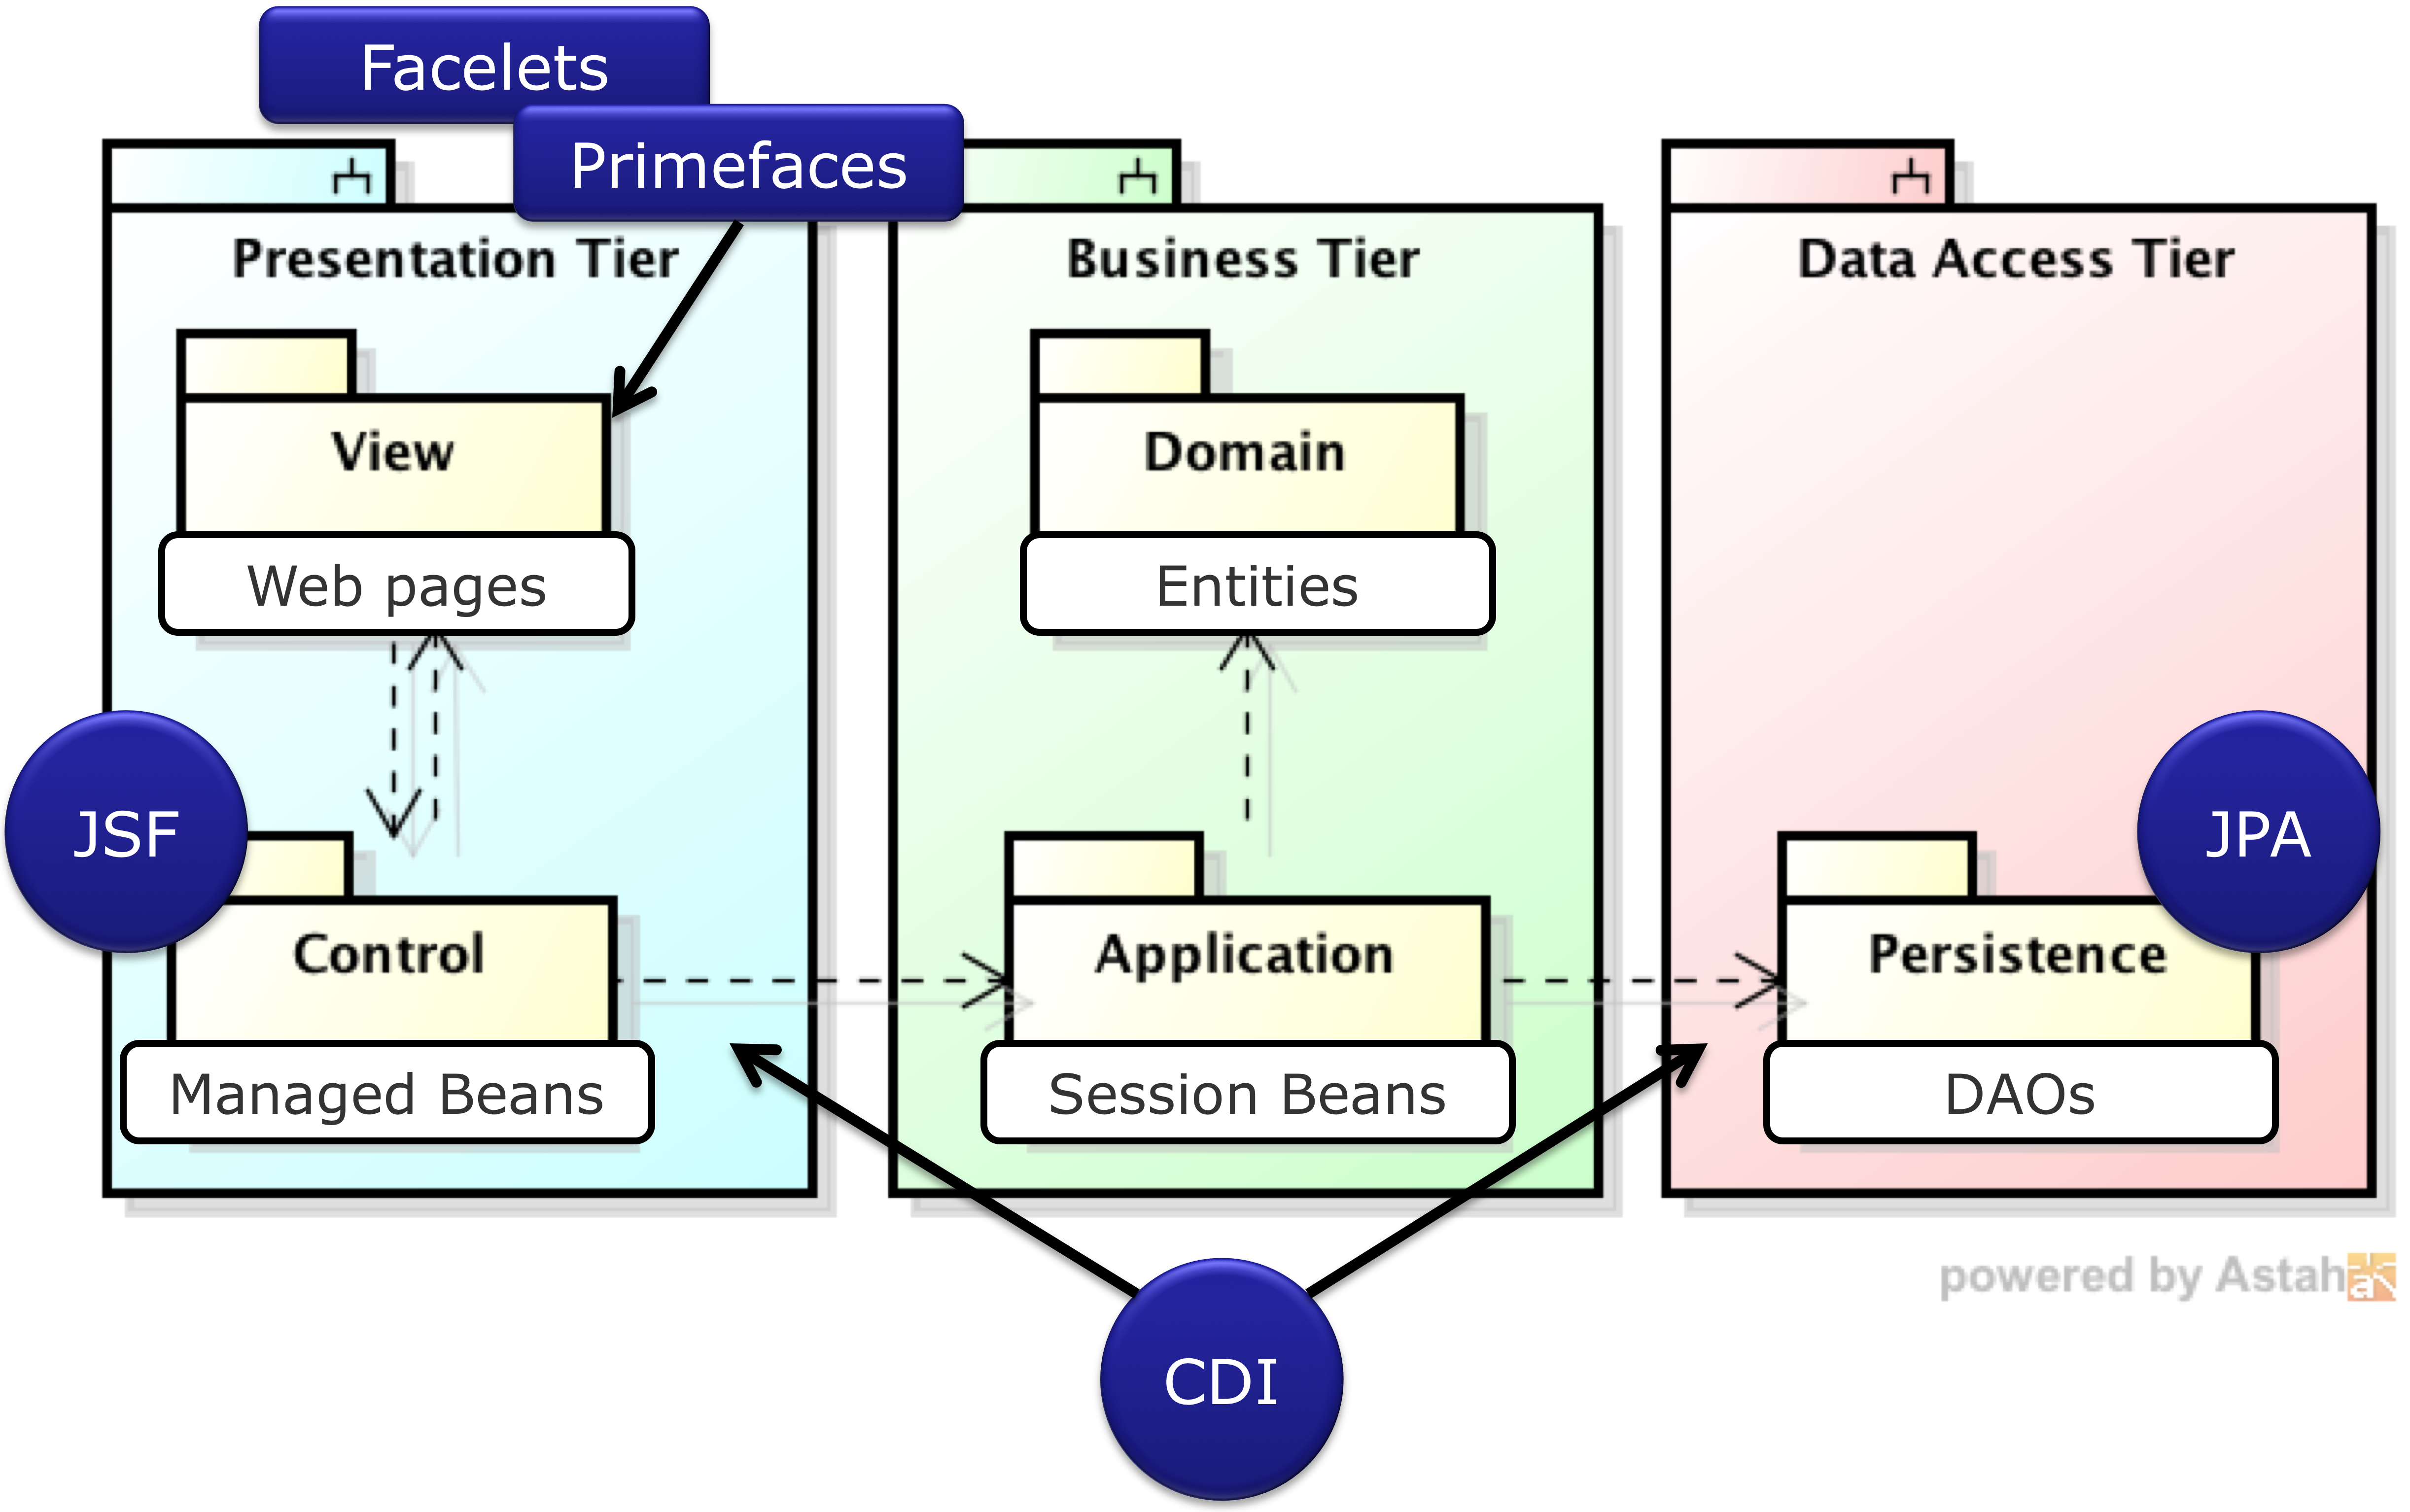
\includegraphics[width=0.9\textwidth]{figuras/figura-arquitetura-padrao.png}
	\caption{Arquitetura padrão proposta pelo FrameWeb~\cite{souza:masterthesis07}.}
	\label{figura-arquitetura-padrao}
\end{figure}

Nas próximas seções, serão apresentados diagramas FrameWeb relativos a cada uma das camadas da arquitetura do sistema.


\section{Camada de Apresentação}
\label{sec-arquitetura-apresentacao}

%\vitor{Apresentar os modelos de navegação do FrameWeb.}

Possui a responsabilidade de realizar a interação entre o sistema e o usuário, exibindo as informações e interpretando os comandos em ações da persistência de dados e da lógica de negócio. Apresenta os modelos de navegação, que auxiliam os desenvolvedores na implementação dos componentes e das classes dos pacotes Visão e Controle.

Os Modelos de Navegação foram gerados de acordo com os casos de uso do sistema. A Figura~\ref{figura-arquitetura-cadastrarUsuarioProfessor} e a Figura~\ref{figura-arquitetura-cadastrarUsuarioSecretario} representam o caso de uso ``Cadastrar Usuário'', que é realizado por um secretário. O caso de uso ``Cadastrar Chefe do Departamento'' também é utilizado por um secretário e foi representado através da Figura~\ref{figura-arquitetura-cadastrarChefeDepartamento}.  

\begin{figure}[h]
	\centering
	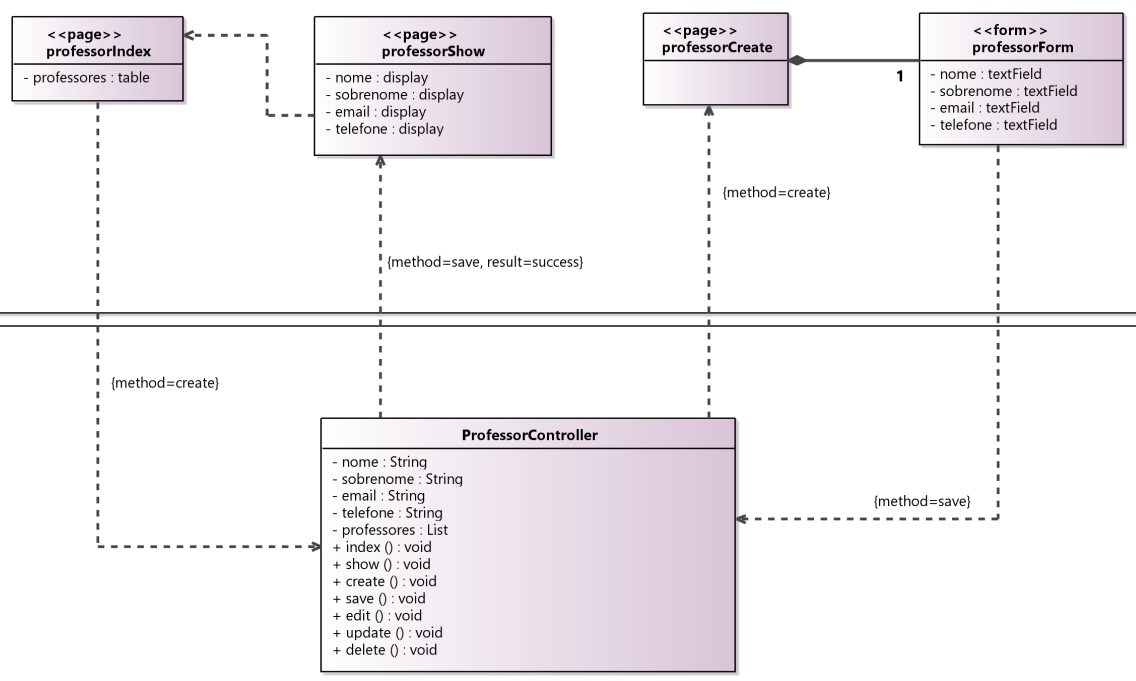
\includegraphics[width=1\textwidth]{figuras/figura-arquitetura-cadastrarUsuarioProfessor.png}
	\caption{Modelo de Navegação do Caso de Uso: Cadastrar Usuário - Professor.}
	\label{figura-arquitetura-cadastrarUsuarioProfessor}
\end{figure}

\begin{figure}[h]
	\centering
	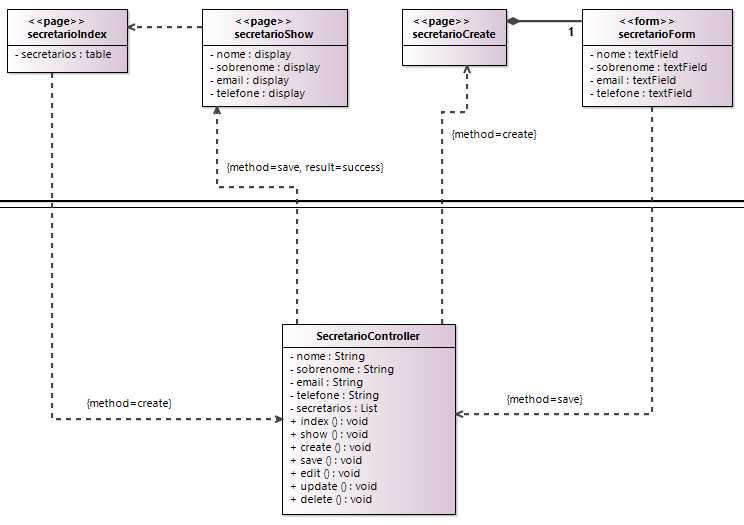
\includegraphics[width=1\textwidth]{figuras/figura-arquitetura-cadastrarUsuarioSecretario.png}
	\caption{Modelo de Navegação do Caso de Uso: Cadastrar Usuário - Secretário.}
	\label{figura-arquitetura-cadastrarUsuarioSecretario}
\end{figure}

\begin{figure}[h]
	\centering
	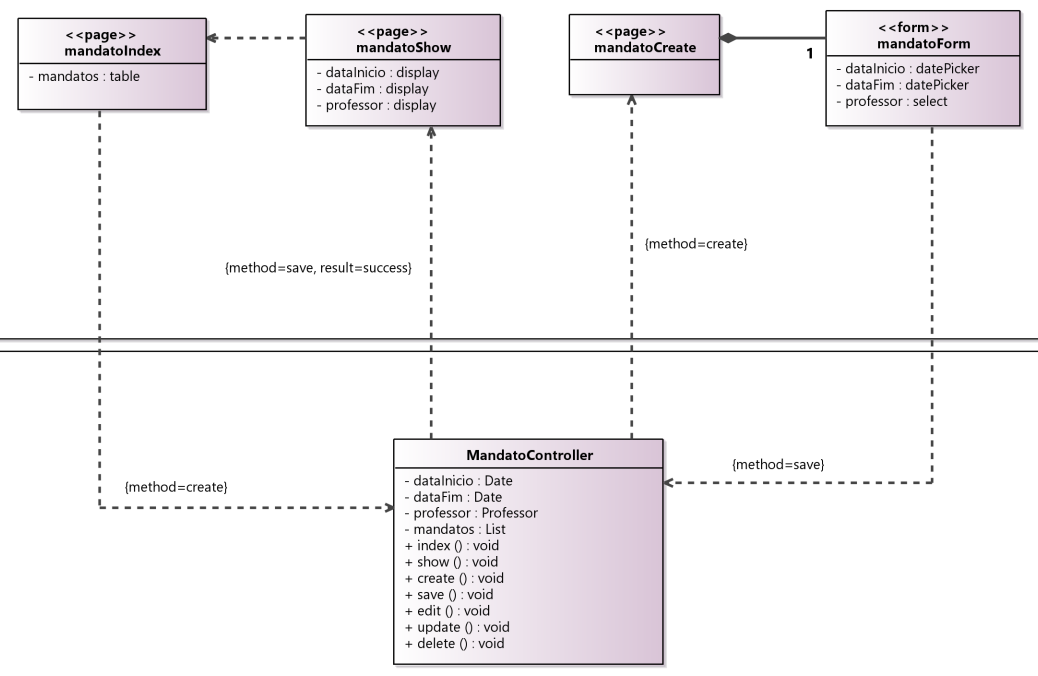
\includegraphics[width=1\textwidth]{figuras/figura-arquitetura-cadastrarChefeDepartamento.png}
	\caption{Modelo de Navegação do Caso de Uso: Cadastrar Chefe do Departamento.}
	\label{figura-arquitetura-cadastrarChefeDepartamento}
\end{figure}

A Figura~\ref{figura-arquitetura-solicitarAfastamento} representa o caso de uso ``Solicitar Afastamento'', que acontece quando um professor realiza o cadastro de um pedido de afastamento. Caso exista um pedido de afastamento internacional, o chefe do departamento utiliza o caso de uso ``Encaminhar Afastamento'', que pode ser visualizado na Figura~\ref{figura-arquitetura-encaminharAfastamento}. 

\begin{figure}[h]
	\centering
	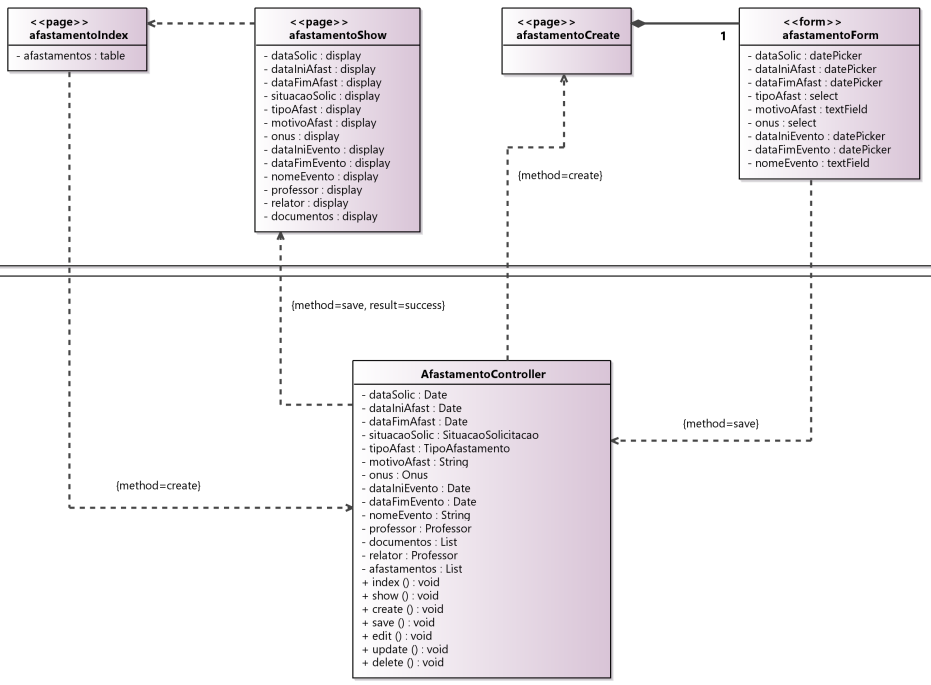
\includegraphics[width=1\textwidth]{figuras/figura-arquitetura-solicitarAfastamento.png}
	\caption{Modelo de Navegação do Caso de Uso: Solicitar Afastamento.}
	\label{figura-arquitetura-solicitarAfastamento}
\end{figure}

\begin{figure}[h]
	\centering
	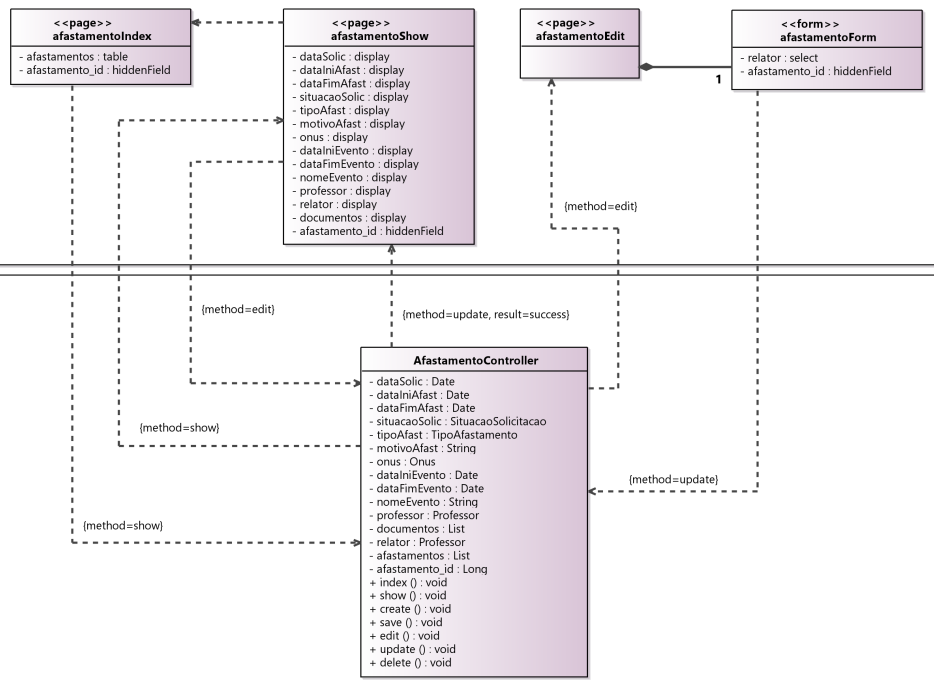
\includegraphics[width=1\textwidth]{figuras/figura-arquitetura-encaminharAfastamento.png}
	\caption{Modelo de Navegação do Caso de Uso: Encaminhar Afastamento.}
	\label{figura-arquitetura-encaminharAfastamento}
\end{figure}

Os casos de uso ``Deferir Parecer'' e ``Manifestar-se Contra Afastamento'' são bem parecidos, pois é necessário realizar o cadastro de um parecer. Portanto, eles foram representados através da Figura~\ref{figura-arquitetura-defParecer_manifContra}. 

\begin{figure}[h]
	\centering
	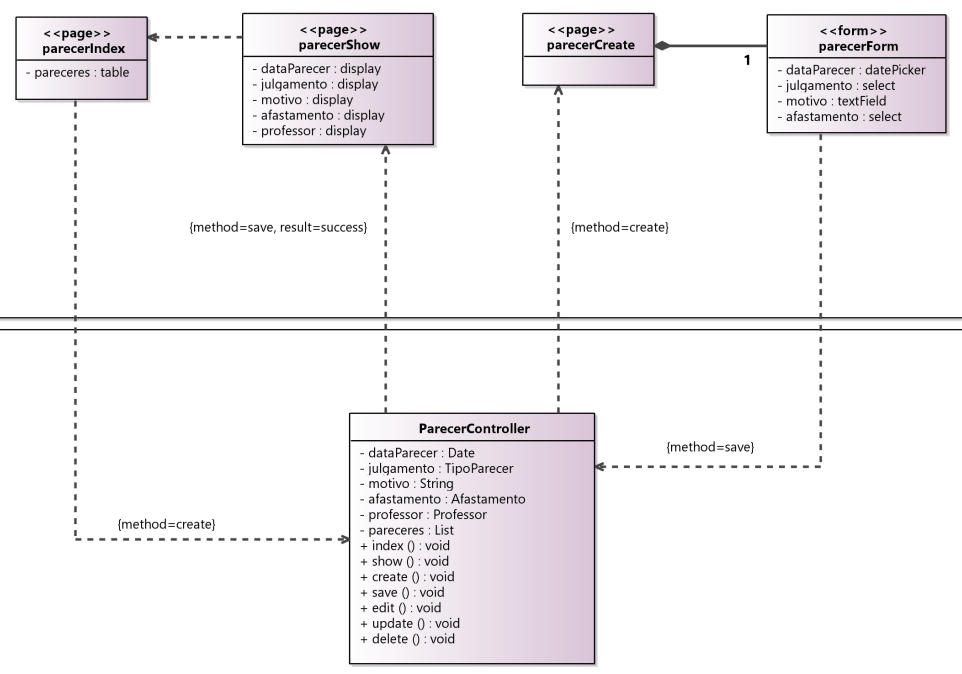
\includegraphics[width=1\textwidth]{figuras/figura-arquitetura-defParecer_manifContra.png}
	\caption{Modelo de Navegação dos Casos de Uso: Deferir Parecer e Manifestar-se Contra Afastamento.}
	\label{figura-arquitetura-defParecer_manifContra}
\end{figure}

Os casos de uso ``Cancelar Afastamento'', ``Arquivar Afastamento'', ``Registrar Parecer CT'' e ``Registrar Parecer PRPPG'' também são bem parecidos. Um professor cancela um pedido de afastamento realizando a alteração da situação da solicitação. Do mesmo modo, um secretário realiza a mudança da situação da solicitação, quando necessita arquivar um afastamento, registrar um parecer do CT ou registrar um parecer da PRPPG. Assim, esses casos de uso foram apresentados na Figura~\ref{figura-arquitetura-cancelar_arquivar_CT_PRPPG}.   

\begin{figure}[h]
	\centering
	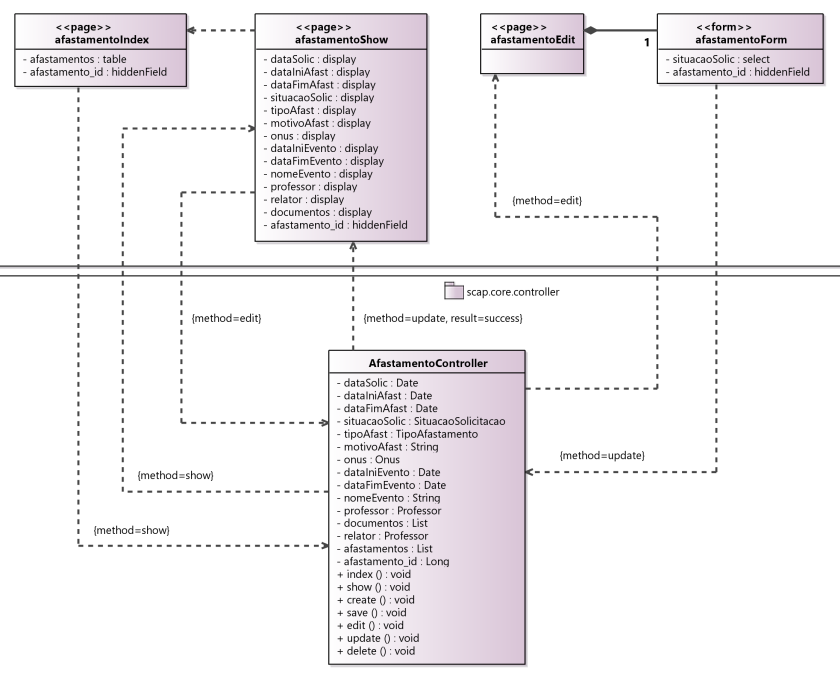
\includegraphics[width=1\textwidth]{figuras/figura-arquitetura-cancelar_arquivar_CT_PRPPG.png}
	\caption{Modelo de Navegação dos Casos de Uso: Cancelar Afastamento, Arquivar Afastamento, Registrar Parecer CT e Registrar Parecer PRPPG.}
	\label{figura-arquitetura-cancelar_arquivar_CT_PRPPG}
\end{figure}

Todos os usuários do sistema podem utilizar o caso de uso ``Consultar Afastamento''. Para isso, é possível filtrar a lista de afastamentos através de quatro buscas diferentes. O caso de uso está representado através da Figura~\ref{figura-arquitetura-consultarAfastamento}.

\begin{figure}[h]
	\centering
	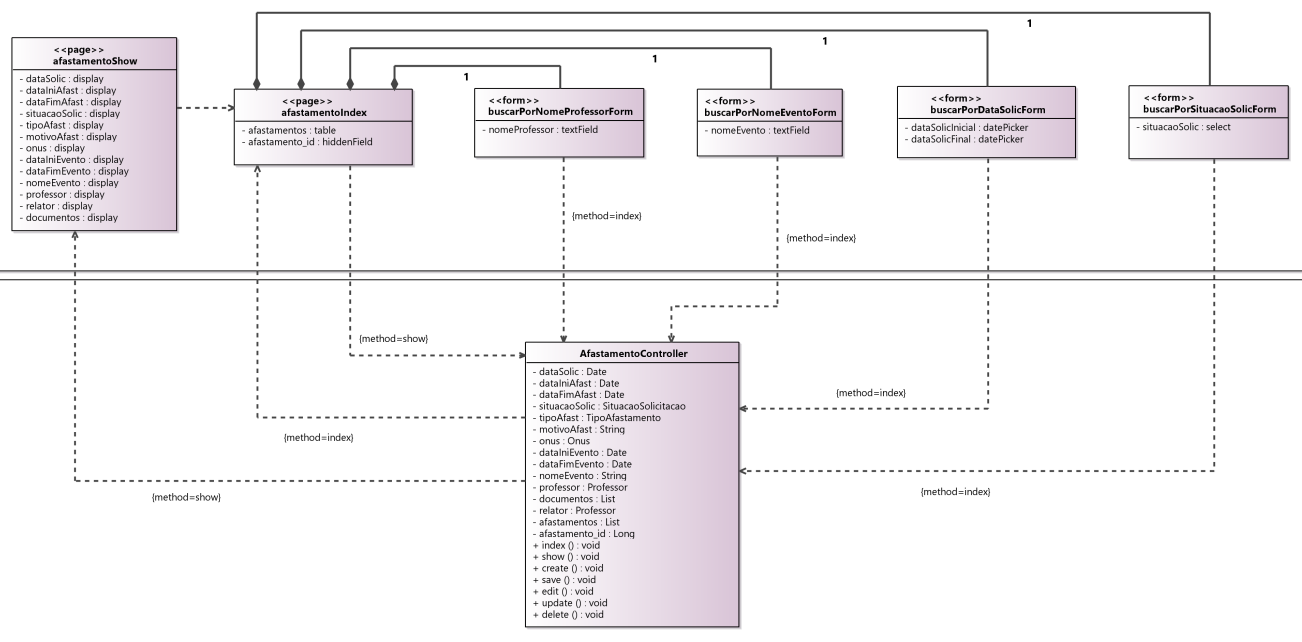
\includegraphics[width=1\textwidth]{figuras/figura-arquitetura-consultarAfastamento.png}
	\caption{Modelo de Navegação do Caso de Uso: Consultar Afastamento.}
	\label{figura-arquitetura-consultarAfastamento}
\end{figure}


\section{Camada de Negócio}
\label{sec-arquitetura-negocio}

%\vitor{Apresentar os modelos de entidades e de aplicação do FrameWeb.}

Engloba as funcionalidades que dão suporte aos processos de negócio, concentrando as regras de negócio, conceitos do domínio, cálculos e processamentos. Representado por um diagrama de classes da UML, o Modelo de Entidades apresenta o mapeamento dos objetos de domínio do problema para a persistência em banco de dados relacional. Esse modelo pode ser visualizado na Figura \ref{figura-arquitetura-entidade} e na Figura \ref{figura-arquitetura-enum}.  

\begin{figure}[h]
	\centering
	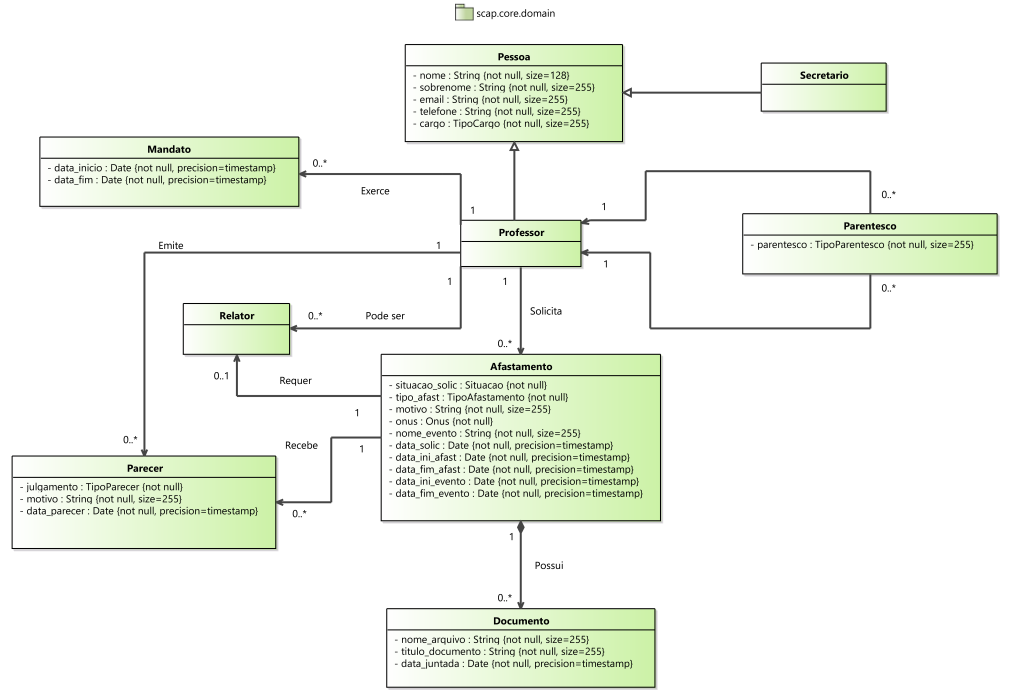
\includegraphics[width=1\textwidth]{figuras/figura-arquitetura-entidade.png}
	\caption{Modelo de Entidades.}
	\label{figura-arquitetura-entidade}
\end{figure}

\begin{figure}[h]
	\centering
	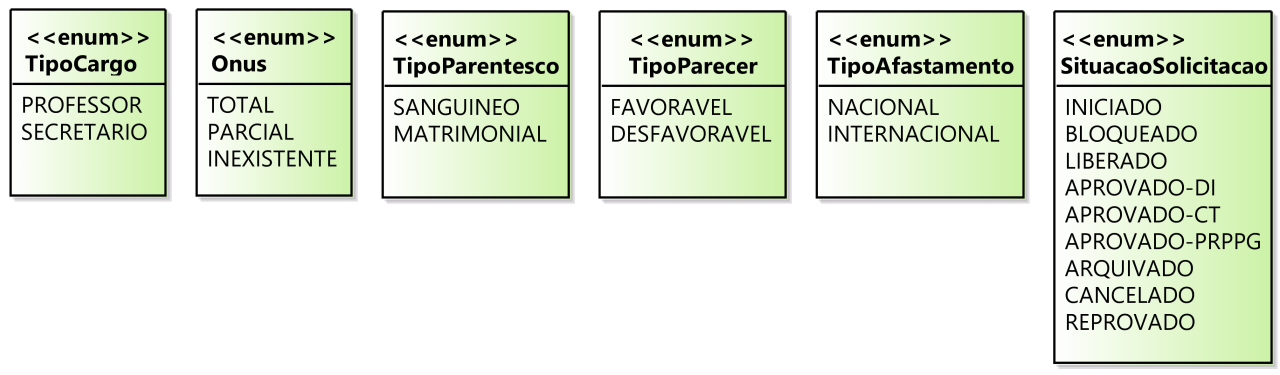
\includegraphics[width=1\textwidth]{figuras/figura-arquitetura-enum.png}
	\caption{Tipos Enumerados do SCAP.}
	\label{figura-arquitetura-enum}
\end{figure}

O diagrama do Modelo de Aplicação é utilizado para auxiliar os desenvolvedores na implementação das classes do pacote Aplicação e na configuração das dependências entre os pacotes Controle, Aplicação e Persistência. Neste projeto foi gerado um modelo de aplicação que representa quais classes de ação que dependem de quais classes de serviço e quais \textit{Data Access Object} (DAO) foram utilizados. Portanto, este modelo pode ser visualizado através da Figura~\ref{figura-arquitetura-aplicacao1} e da Figura~\ref{figura-arquitetura-aplicacao2}. 

\begin{figure}[h]
	\centering
	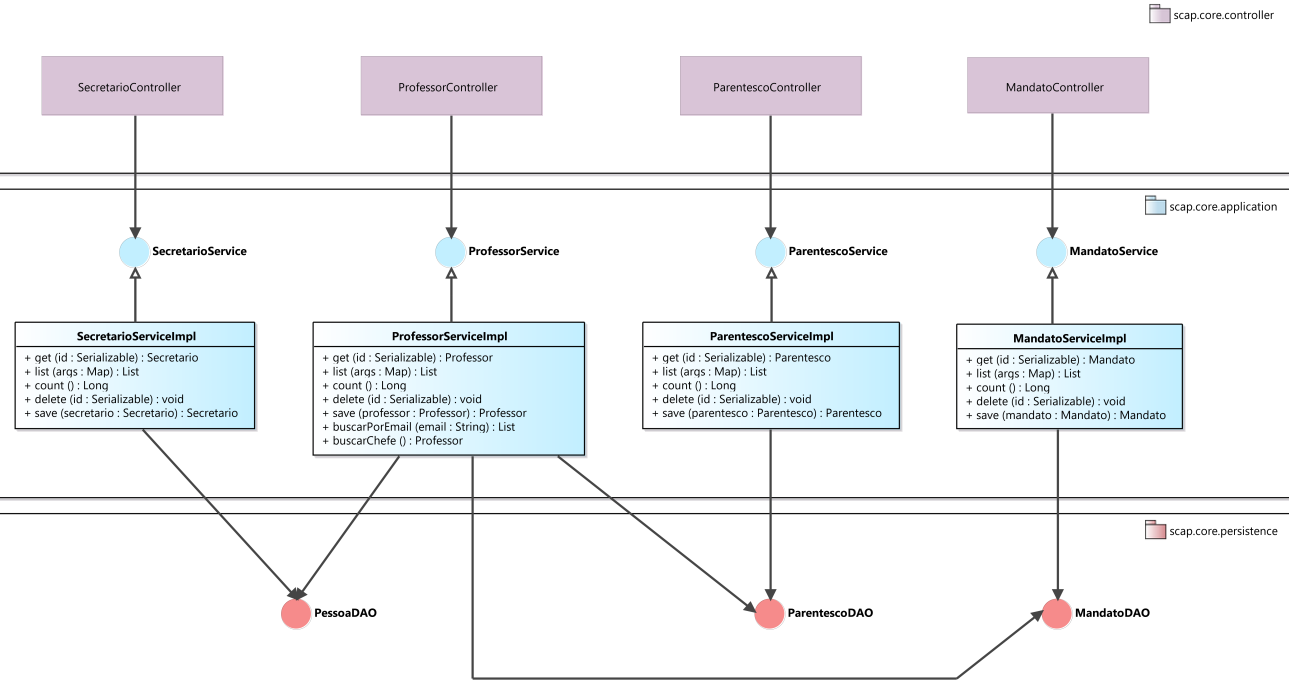
\includegraphics[width=1\textwidth]{figuras/figura-arquitetura-aplicacao1.png}
	\caption{Modelo de Aplicação - Parte 1.}
	\label{figura-arquitetura-aplicacao1}
\end{figure}

\begin{figure}[h]
	\centering
	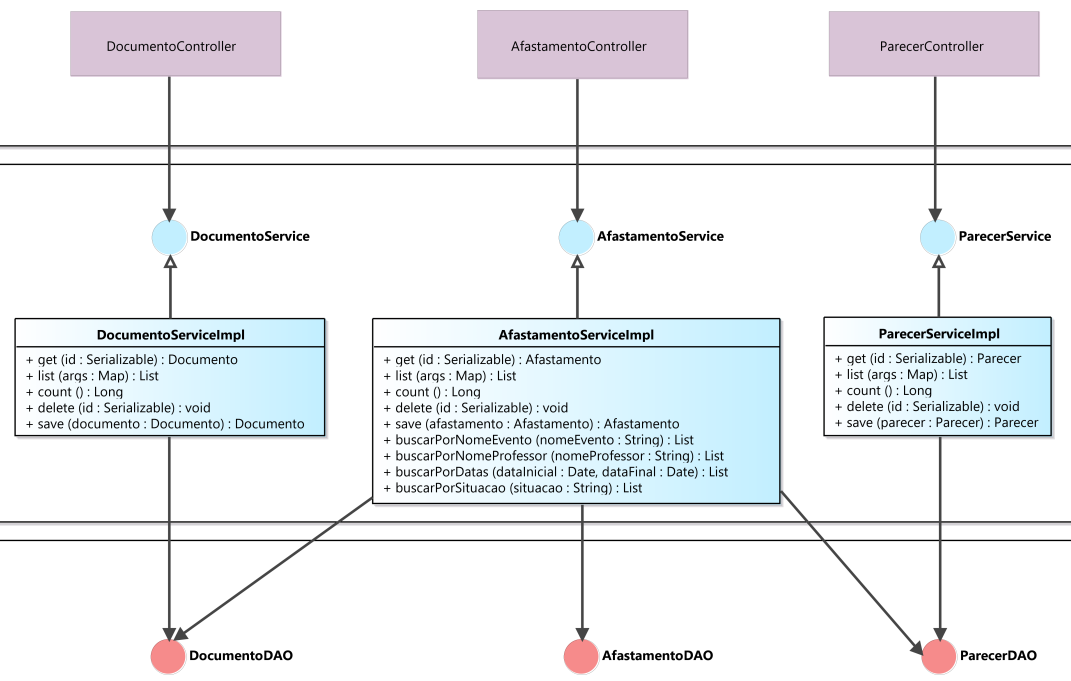
\includegraphics[width=1\textwidth]{figuras/figura-arquitetura-aplicacao2.png}
	\caption{Modelo de Aplicação - Parte 2.}
	\label{figura-arquitetura-aplicacao2}
\end{figure}


\section{Camada de Acesso a Dados}
\label{sec-arquitetura-dados}

%\vitor{Apresentar os modelos de persistência do FrameWeb.}

Estabelece o acesso a dados, gerenciando requisições e cuidando da sincronização de elementos de dados. Um diagrama de classes da UML representa as classes DAO existentes, que são responsáveis pela persistência das instância das classes de domínio. Esse diagrama pode ser visualizado na Figura \ref{figura-arquitetura-persistencia}.

Com o intuito de não causar poluição visual, é possível fazer com que os métodos que são comuns a todas a interfaces DAOs não sejam repetidos sem necessidade. Para isso, basta apresentar DAOs base que declaram esses métodos. De forma automática, todas as interfaces DAO de todos os diagramas herdam as definições da interface base, ocorrendo o mesmo com as implementações concretas de cada tecnologia de persistência, sem que isso precise estar explícito no diagrama. Ainda é possível declarar tanto a interface quanto a classe DAOBase usando tipos genéricos, deixando a cargo de suas sub-interfaces e sub-classes a especificação da classe gerenciada por cada DAO~\cite{souza:masterthesis07}. 

\begin{figure}[h]
	\centering
	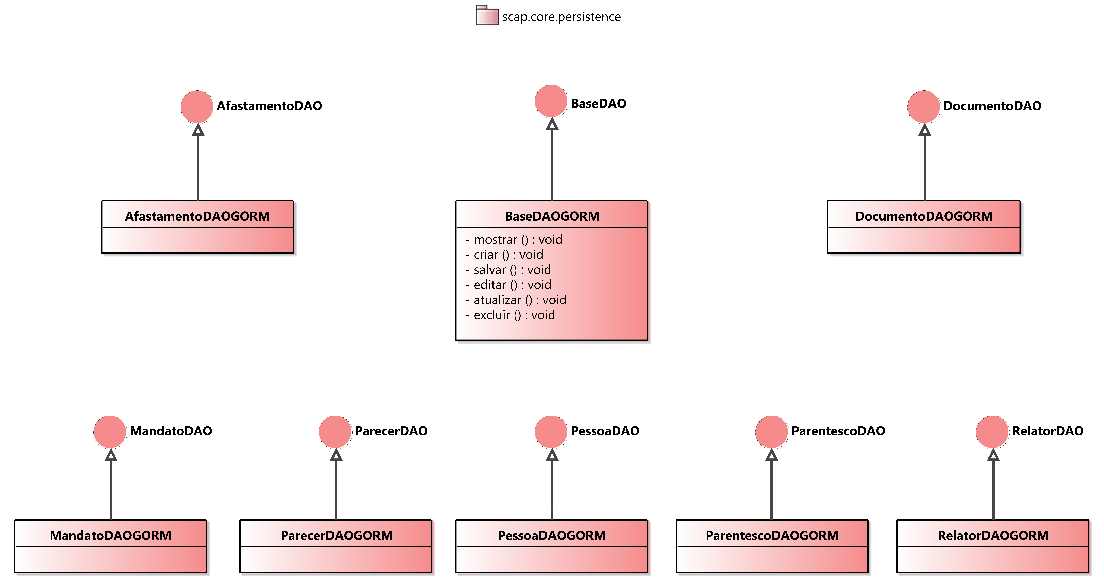
\includegraphics[width=1\textwidth]{figuras/figura-arquitetura-persistencia.png}
	\caption{Modelo de Persistência.}
	\label{figura-arquitetura-persistencia}
\end{figure}
